\documentclass[12pt,a4paper]{report}
\usepackage{amsmath}
\usepackage{amsfonts}
\usepackage{amssymb}
\usepackage{fullpage}
\usepackage[slovak]{babel}
\usepackage[utf8]{inputenc}
\usepackage[T1]{fontenc}
\usepackage{fullpage}
\usepackage{indentfirst}
\usepackage{array}
\usepackage{graphicx}
\usepackage{caption}
\usepackage{placeins}
\DeclareGraphicsExtensions{.png,.jpg}

\begin{document}
\begin{titlepage}
\centering\bfseries
		Fakulta matematiky, fyziky a informatiky\\Univerzita Komenského v Bratislave	
	\vspace*{\stretch{2.0}}

	\fontsize{23}{28}\textbf{Špecifikácia požiadaviek na softvér}\\
	\vspace*{\stretch{0.05}}
	\fontsize{16}{22}\textbf{Predikcia šírenia infekčných ochorení}\\
	\vspace*{\stretch{0.2}}
	\large\textit{Matúš Čongrády\\Tibor Hanesz\\Katarína Šimnová}

	\vspace*{\stretch{2.0}}
\end{titlepage}\bigskip
	\setcounter{tocdepth}{9}
	\tableofcontents

\renewcommand{\chaptername}{}	
\chapter[Konceptuálna analýza]{\rmfamily\bfseries
	Konceptuálna analýza}

\section[Používateľské rozhranie]{\rmfamily\bfseries
	Používateľské rozhranie}
Táto  časť  bude  venovaná približnému  grafickému  opisu užívateľského  rozhrania. Opisuje aké komponenty sa budú nachádzať na akých stránkach a čo bude ich želaným vstupom.

\subsection[Hlavná stránka]{\rmfamily\bfseries
	Hlavná stránka}

\begin{figure}[htb]
	\centering
	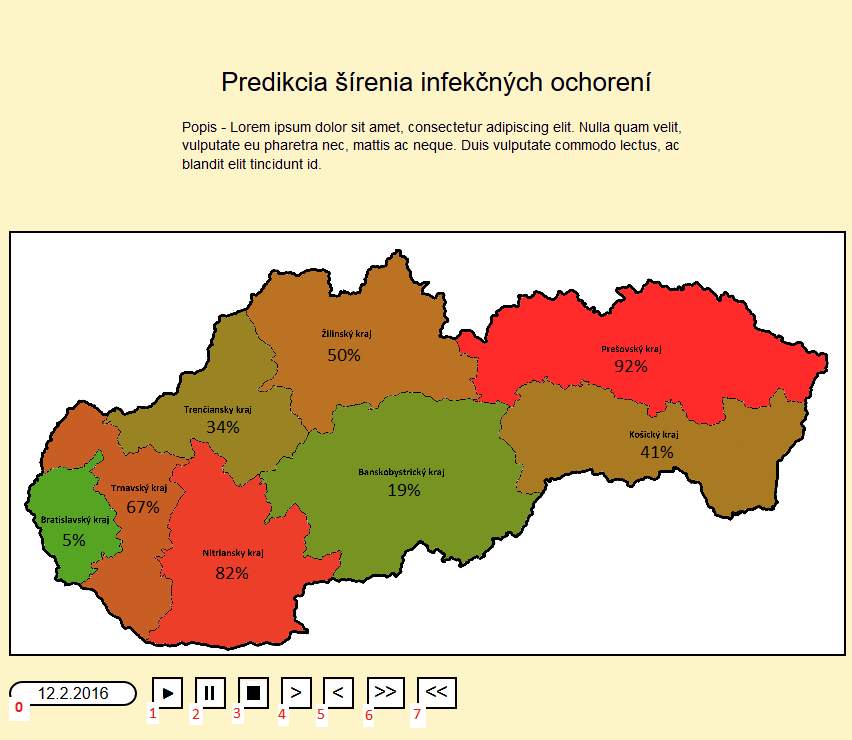
\includegraphics[scale=0.55]{hl_stranka}
	\caption{Hlavná stránka}
	\label{fig:Hlavná stránka}
\end{figure}


\begin{table}[h!]
	\centering
	\begin{tabular}{|>{\centering\arraybackslash}m{3in}|>{\centering\arraybackslash}m{3in}|}
		\hline
		\centering Parameter & Vlastnosti \\ [0ex]
		\hline
		Mapa & Miesto zobrazenia animácie šírenia infekčného ochorenia.\\ [0ex]
		\hline
		0. &  Označuje deň, pre ktorý animácia v danom momente zobrazuje štatistiku.\\ [0ex]
		\hline
		1. & Spustenie animácie.\\ [0ex]	
		\hline
		2. & Zastavenie animácie.\\ [0ex]	
		\hline
		3. & Vypnutie animácie.\\ [0ex]	
		\hline
		4. & Prechod o jeden deň vpred.\\ [0ex]	
		\hline
		5. & Prechod o jeden deň vzad.\\ [0ex]	
		\hline
		6. & Zrýchlenie animácie.\\ [0ex]	
		\hline
		7. & Spomalenie animácie.\\ [0ex]	
		\hline
		
	\end{tabular}
\end{table}
\FloatBarrier
\pagebreak
\subsection[Prihlásenie]{\rmfamily\bfseries
	Prihlásenie}

\begin{figure}[htb]
	\centering
	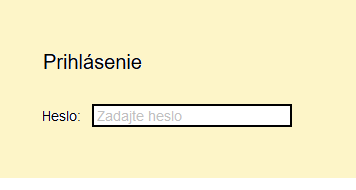
\includegraphics[scale=0.6]{prihlasenie}
	\caption{Prihlásenie}
	\label{fig:Prihlásenie}
\end{figure}


\begin{table}[h!]
	\centering
	\begin{tabular}{|>{\centering\arraybackslash}m{3in}|>{\centering\arraybackslash}m{3in}|}
		\hline
		\centering Parameter & Vlastnosti \\ [0ex]
		\hline
		Heslo & Užívateľ zadá svoje prihlasovacie heslo. \\ [0ex]
		\hline
	\end{tabular}
\end{table}
\FloatBarrier
\subsection[Administrácia]{\rmfamily\bfseries
	Administrácia}

\begin{figure}[!h]
	\centering
	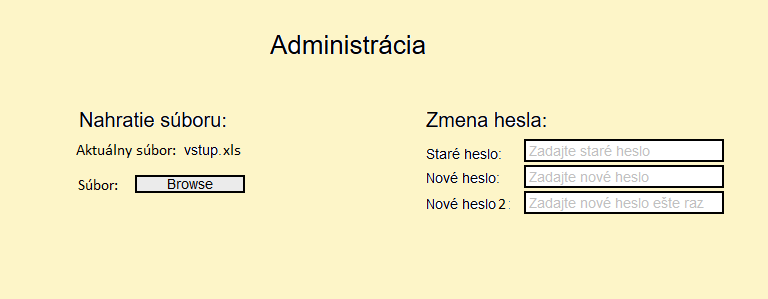
\includegraphics[scale=0.7]{admin}
	\caption{Administrácia}
	\label{fig:Administrácia}
\end{figure}

\begin{table}[h!]
	\centering
	\begin{tabular}{|>{\centering\arraybackslash}m{3in}|>{\centering\arraybackslash}m{3in}|}
		\hline
		\centering Parameter & Vlastnosti \\ [0ex]
		\hline
		Aktuálny súbor & Návestie zobrazujúce názov súboru aktuálne použitého vstupu.\\ [0ex]
		\hline
		Súbor & Užívateľ vyberie validný XLS alebo XLSX súbor obsahujúci maticu. \\ [0ex]
		\hline
		Staré heslo & Užívateľ zadá svoje pôvodné heslo.\\ [0ex]	
		\hline
		Nové heslo & Užívateľ zadá svoje nové heslo. \\ [0ex]		
		\hline
		Nové heslo 2 & Užívateľ zadá svoje nové heslo druhýkrát. \\ [0ex]		
		\hline
	\end{tabular}
\end{table}
\FloatBarrier
\pagebreak
\section[Možnosti užívateľa]{\rmfamily\bfseries
	Možnosti užívateľa}

V tejto časti sú umiestnené diagramy, ktoré popisujú predovšetkým možné činnosti užívateľa resp. administrátora v systéme.

\subsection[Stavový diagram]{\rmfamily\bfseries
	Stavový diagram}
Tento diagram ukazuje jednotlivé stavy a ich zmeny v troch situáciách:
\begin{itemize}
	\item prezeranie prezentácie,
	\item zmena hesla,
	\item zmena údajov, z ktorých sa vytvára animácia.
\end{itemize}
\begin{figure}[htb]
	\centering
	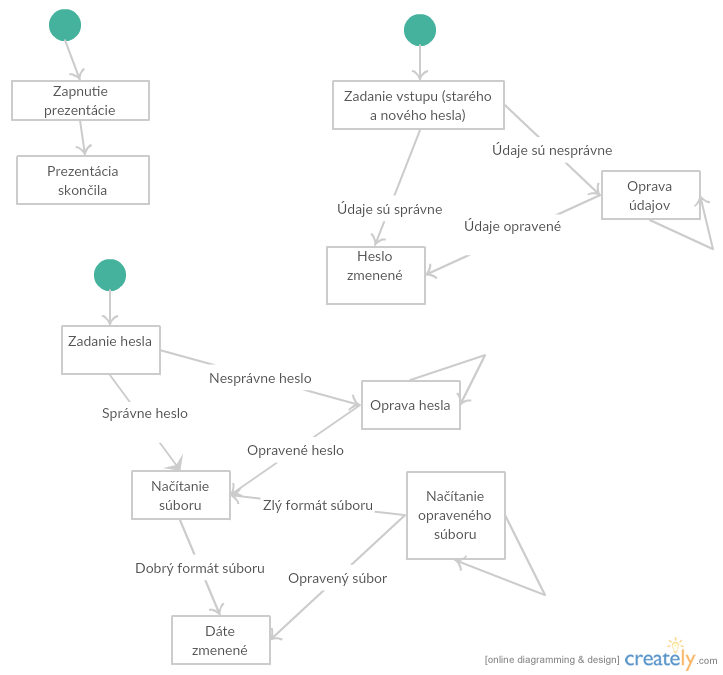
\includegraphics[scale=0.5]{Stavovy_diagram}
	\caption{Stavový diagram}
	\label{fig:Stavový diagram}
\end{figure}
\FloatBarrier
\clearpage
\subsection[Use case diagram]{\rmfamily\bfseries
	Use case diagram}
Tento diagram poskytuje najzákladnejší prehľad prípadov použitia. Každý prípad použitia opisuje jeden spôsob použitia systému z hľadiska používateľa.

\begin{figure}[htb]
	\centering
	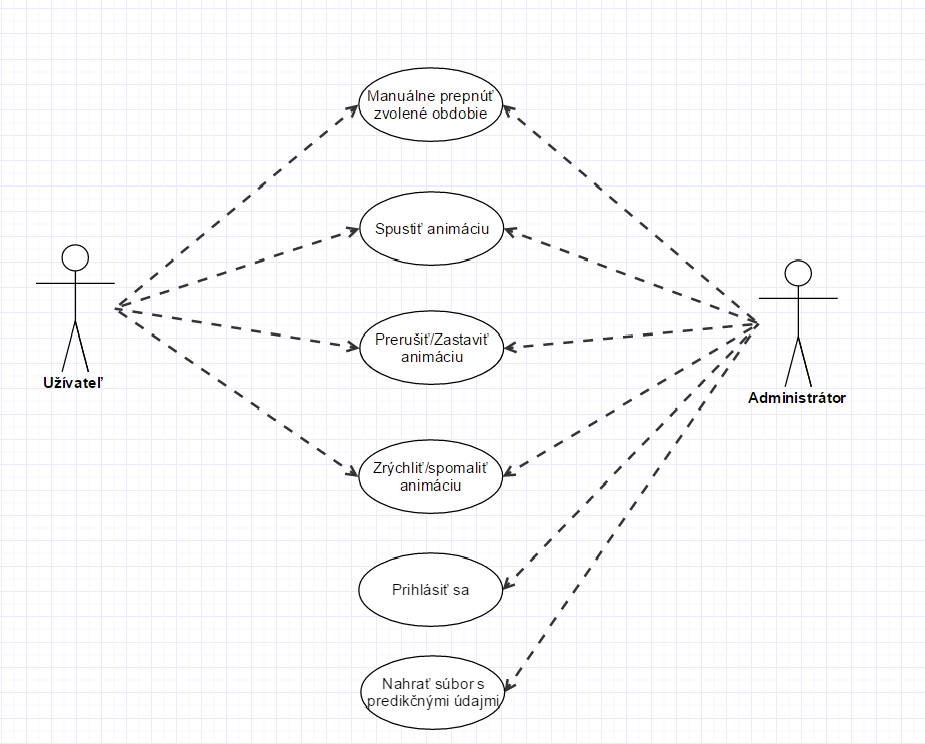
\includegraphics[scale=0.6]{use_case_diagram}
	\caption{Use case diagram}
	\label{fig:Use case diagram}
\end{figure}


\FloatBarrier
\clearpage
\subsection[Entito-relačný diagram]{\rmfamily\bfseries
	Entito-relačný diagram}
Tento diagram je vlastne špeciálnym grafom, ktorý naznačuje vzťahy medzi subjektami v databáze.

\begin{figure}[htb]
	\centering
	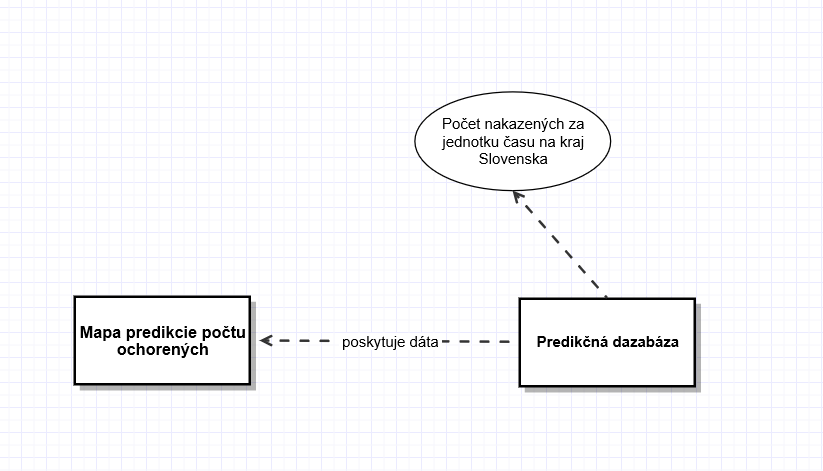
\includegraphics[scale=0.7]{E-R_diagram}
	\caption{Entito-relačný diagram}
	\label{fig:Entito-relačný diagram}
\end{figure}

\FloatBarrier

\renewcommand{\chaptername}{}	
\chapter[Analýza technológií, dekompozícia a dátový model]{\rmfamily\bfseries
	Analýza technológií, dekompozícia a dátový model}
	

\section[Možné použité technológie a postupy]{\rmfamily\bfseries
	Možné použité technológie a postupy}

\subsection[Technológie]{\rmfamily\bfseries
	Technológie}
Na strane servera sme sa rozhodli použiť server nginx a PHP. Nginx preto, lebo nie je tak robustný, je stále pravidelne podporovaný a taktiež nezávislý od jedného operačného systému. PHP sme zvolili kvôli jednoduchosti, ľahkému nasadeniu, osobnej preferencie a skúsenosti a vzhľadom na jednoduchosť nie je potrebné hľadieť na rýchlosť do detailov. Na čítanie súborov z excelu použijeme voľne dostupnú knižnicu PHPExcel.
\par
Na strane klienta použije HTML5 a CSS3 na layout. Okrem toho použijeme JavaScript a knižnicu jQuery spolu s nadstavbou pre validáciu pre komfortnejšie užívateľské rozhranie. Tieto technológie sme zvolili vzhľadom na rozšírenosť, osobnú preferenciu a skúsenosť. 
\par
Na vykreslenie mapy použijeme Google Map API v3. Je to najrozšírenejšie maps API, ktoré nám ponúka presne tú funkcionalitu, ktorú potrebujeme.
\pagebreak

\section[Deployment diagram]{\rmfamily\bfseries
	Deployment diagram}
Prichádzajúce HTTP požiadavky vyhodnotí najprv nginx server a následne PHP. Posiela statický obsah ako HTML, CSS, JavaScript a obrázky. Taktiež posiela dáta na vytvorenie animácie prostredníctvom métody POST.
\begin{figure}[htb]
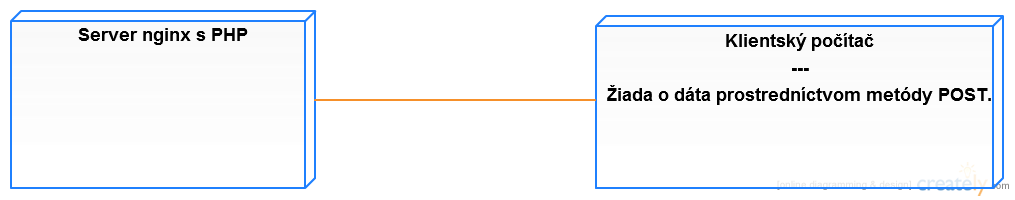
\includegraphics[scale=0.5]{deployment}
\caption[Deployment diagram]{Deployment diagram}
 \label{fig:Deployment diagram}
\end{figure}


\section[Domain model diagram]{\rmfamily\bfseries
	Domain model diagram}
Administrátor (zadávateľ) uploadne na stránku .xls súbor, ktorý server spracuje a uloží si z neho dáta. Štruktúra uloženého údaju - počet ochorených / deň / kraj Slovenska. Server spracuje požiadavky od užívateľa a pošle statický obsah stránky. Webová stránka následne zobrazí animáciu pre užívateľa.
\begin{figure}[htb]
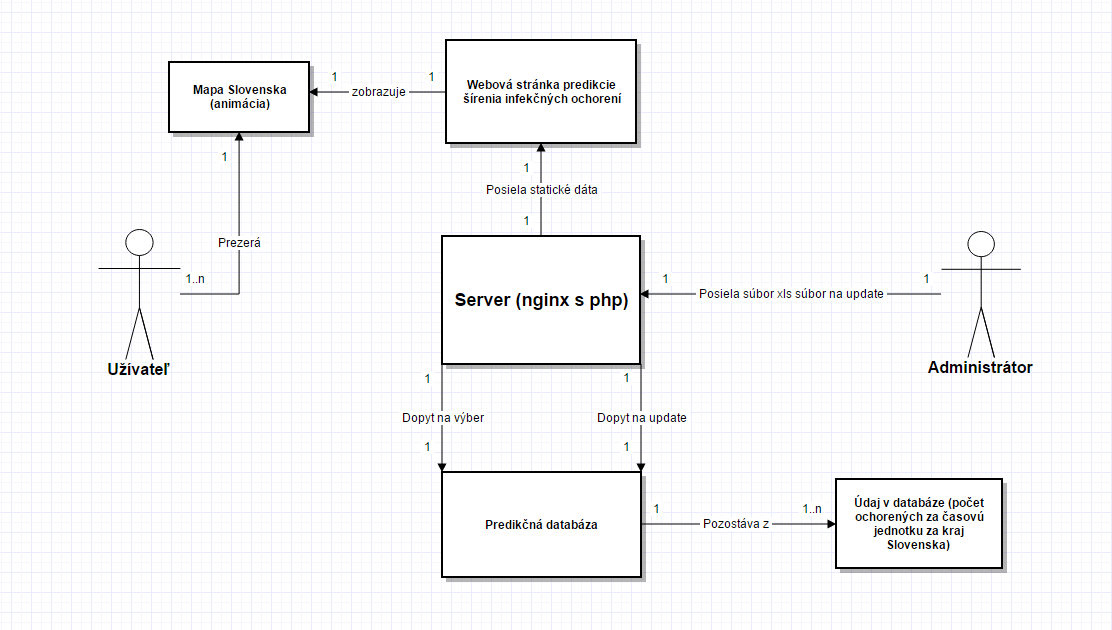
\includegraphics[scale=0.5]{Domain_model_diagram}
\caption[Domain model diagram]{Domain model diagram}
 \label{fig:Domain model diagram}
\end{figure}

\section[Data model]{\rmfamily\bfseries
	Data model}
Administrátor (zadávateľ) uploadne na stránku .xls alebo .xlsx súbor, ktorý server spracuje. Server dáta prekonvertuje do formátu JSON. Následne ich uloží do .json súboru, ktorý sa nachádza na serveri. Relatívna cesta k súboru: ../data/data.json
\begin{figure}[htb]
	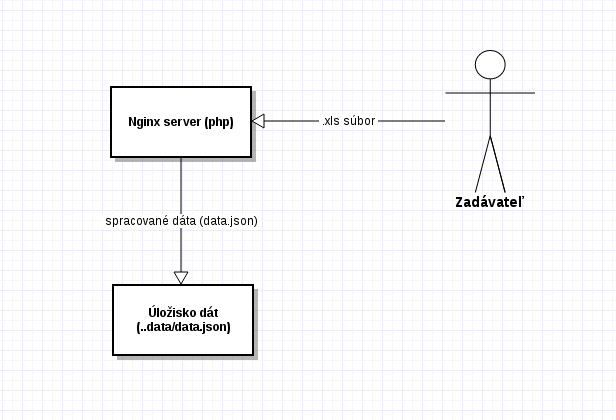
\includegraphics[scale=0.5]{data_model}
	\caption[Data model]{Data model}
	\label{fig:Data model}
\end{figure}


\renewcommand{\chaptername}{}	
\chapter[Návrh]{\rmfamily\bfseries
	Návrh}

\section[Modelové triedy]{\rmfamily\bfseries
	Modelové triedy}

\subsection[Trieda Administration]{\rmfamily\bfseries
	Trieda Administration}
Atribúty:
\begin{itemize}
		\item FILE – Konštanta obsahujúca názov súboru s údajmi. 
\end{itemize}
Metódy
\begin{itemize}
	\item changePassword(\$oldPassword, \$newPassword, \$newPasswordCheck) – Zmení heslo administrátora, ak je staré heslo správne a ak sú obe nové heslá rovnaké, inak vyhodí error.
	\item uploadFile(\$file) – Prepíše údaje z excel súboru do JSON súboru a zapíše ho na disk.
\end{itemize}

\subsection[Trieda Passwd]{\rmfamily\bfseries
	Trieda Passwd}
Atribúty:
\begin{itemize}
	\item SERCRET\_KEY – Konštanta, ktorá obsahuje tajný kľúč, ktorý sa pripíše k heslu pri vytváraní hešu. 
	\item FILE – Konštanta obsahujúca názov súboru s heslom.
\end{itemize}
Metódy
\begin{itemize}
	\item readFromFile() – Prečíta heslo zo súboru.
	\item createNewPassword(\$passwd) – Zapíše nové heslo do súboru ako heš.
	\item makeHash(\$phrase) – Vytvorí z hesla heš.
	\item comparePasswords(\$passwd) – Porovná zadané heslo s heslom zo súboru.
\end{itemize}

\subsection[Trieda Map]{\rmfamily\bfseries
	Trieda Map}

Metódy
\begin{itemize}
	\item initialize() – Zobrazenie mapy a inicializácia hodnôt.
	\item mapPaint() – Zafarbenie jednotlivých krajov slovenska na mape.
	\item mapStart() – Spustenie animácie.
	\item mapPause() – Pozastavenie animácie.
	\item mapStop() – Zastavenie animácie a pretočenie na začiatok.
	\item mapNext() – Prechod na další obrázok animácie.
	\item mapPrevious() – Prechod na predcháchadzajúci obrázok animácie.
	\item mapFast() – Zrýchlenie animácie.
	\item mapSlow() – Spomalenie animácie.
\end{itemize}

\section[Triedy typu radič]{\rmfamily\bfseries
	Triedy typu radič}

\subsection[Trieda GetDataFromServer]{\rmfamily\bfseries
	Trieda GetDataFromServer}
Metódy
\begin{itemize}
	\item getDataFromServeromFile(successListener, errorListener) – Získa údaje zo servera GET požiadavkou. Dva parametre predstavujú funkcie, čo robiť, ak sme údaje získali úspešne resp. neúspešne.
\end{itemize}

\section[Data flow diagram]{\rmfamily\bfseries
	Data flow diagram}
	Diagram graficky znázorňuje toky údajov prúdiace cez informačný systém. Vizualizuje proces spracovávania údajov.
	
	\begin{figure}[htb]
		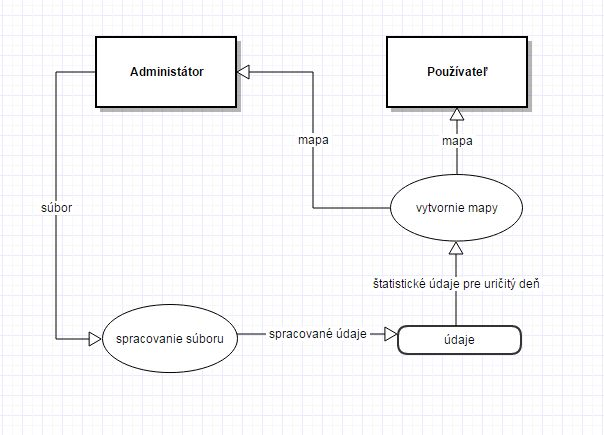
\includegraphics[scale=0.5]{data_flow}
		\caption[Data flow diagram]{Data flow diagram}
		\label{fig:Data flow diagram}
	\end{figure}
\clearpage
\section[Sekvenčný diagram]{\rmfamily\bfseries
		Sekvenčný diagram}
	Diagram zobrazuje postup pri zmene hesla. Užívateľ vyplní staré heslo, nové heslo a nové heslo ešte raz pre kontrolu. Staré heslo sa skontrolouje so serverom a nové heslá sa skontrolujú navzájom. Ak je všetko správne, užíveteľovi sa zmení heslo, inak sa zobrazí chybová hláška a bude možnosť opraviť vstup.
	
	\begin{figure}[htb]
		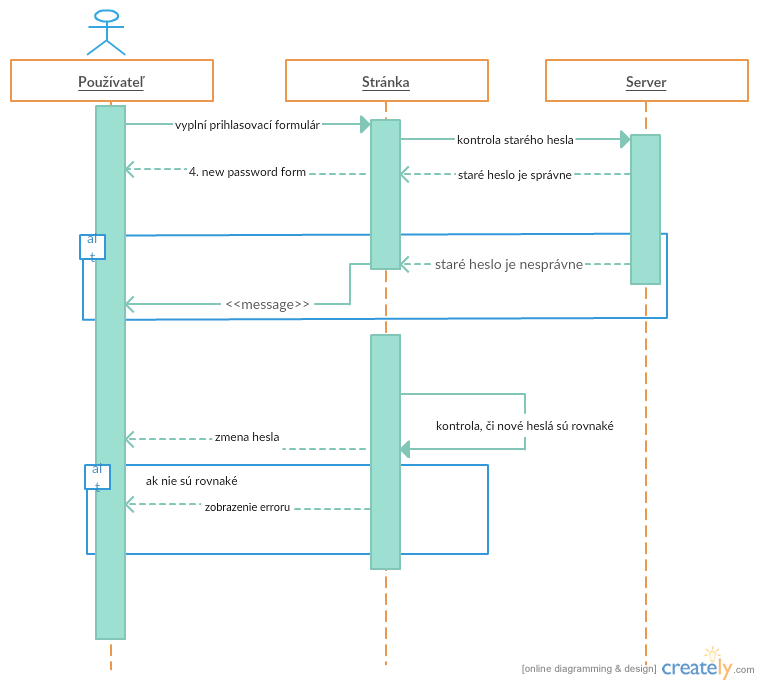
\includegraphics[scale=0.5]{sequence}
		\caption[Data flow diagram]{Sekvenčný diagram}
		\label{fig:Sekvenčný diagram}
	\end{figure}


\chapter[Podrobná špecifikácia komponentov]{\rmfamily\bfseries
	Podrobná špecifikácia komponentov}

\section[Modelové triedy]{\rmfamily\bfseries
	Modelové triedy}

\subsection[Trieda Administration]{\rmfamily\bfseries
	Trieda Administration}
Atribúty:
\begin{itemize}
	\item FILE – Konštana obsahujúca názov súboru s údajmi. 
\end{itemize}
Metódy
\begin{itemize}
	\item changePassword(string \$oldPassword, string \$newPassword, string \$newPasswordCheck) – Najprv skontrolouje staré heslo, ak je nesprávne vyhodí chybovú hlášku. Ak je správne skontroluje nové heslá, ak sa zhodujú, tak zmení heslo, tak vyhodí chybovú hlášku.
	\item uploadFile(file \$file) – Najprv skontroluje, či je súbor menší ako 1 megabajt a či má správny formát. Ak áno, pomocou knižnice PHPExcel prečíta daný excelovský súbor. Hondnoty z neho zapisuje do dvojrozmerného poľa, ktoré potom vo formáte JSON zapíše do súboru.
\end{itemize}

\subsection[Trieda Passwd]{\rmfamily\bfseries
	Trieda Passwd}
Atribúty:
\begin{itemize}
	\item SERCRET\_KEY – Konštanta, ktorá obsahuje tajný kľúč, ktorý sa pripíše ku heslo pri vytváraní hešu. 
	\item FILE – Konštana obsahujúca názov súboru s heslom.
\end{itemize}
Metódy
\begin{itemize}
	\item readFromFile() – Prečíta heslo zo súboru alebo vyhodí chybu, ak to nie je možné.
	\item createNewPassword(string \$passwd) – Zapíše nové heslo do súboru ako heš alebo vyhodí chybu, ak to nie je možné.
	\item makeHash(string \$phrase) – Najprv vytvorí soľ tak, že daný string zahešuje algoritmom SHA512 a z neho vezme niektoré znaky. Heš vytvorí ako spojenie tajného kľúča SERCRET\_KEY, \$phrase a soli prostredníctvom algoritmu SHA512.
	\item comparePasswords(string \$passwd) – Prečíta heslo zo súboru pomocou readFromFile() a porovná s \$passwd.
\end{itemize}

\section[Triedy typu radič]{\rmfamily\bfseries
	Triedy typu radič}

\subsection[Trieda GetDataFromServer]{\rmfamily\bfseries
	Trieda GetDataFromServer}
Metódy
\begin{itemize}
	\item getDataFromServeromFile(successListener, errorListener) – Získa údaje zo servera pomocou ajaxu GET požiadavkou v JSON formáte. Dva parametre predstavujú funkcie, čo robiť, ak sme údaje získali úspešne resp. neúspešne.
\end{itemize}

\subsection[Trieda Map]{\rmfamily\bfseries
	Trieda Map}

Metódy
\begin{itemize}
	\item initialize() – Vykreslí SVG mapu, inicializuje parametre mapy, nastaví animáciu do počiatočného stavu.
	\item mapPaint() – Prechádza všetkými krajmi, číta dáta o počte nakazených a zafarbuje kraje prislusnou farbou.
	\item mapStart() – Spustí sa thread animácie, po každom kroku sa prekraslí mapa.
	\item mapPause() – Prerúší sa thread animácie.
	\item mapStop() – Zastaví sa thread animácie a animácia sa pretočí na začiatok.
	\item mapNext() – Vykreslia sa farby krajov pre další deň.
	\item mapPrevious() – Vykreslia sa farby krajov pre predchádzajúci deň.
	\item mapFast() – Beh threadu sa zrýchli.
	\item mapSlow() – Beh threadu sa spomalí.
\end{itemize}

\chapter[Testovacie scenáre]{\rmfamily\bfseries
	Testovacie scenáre}

\section[Zmena hesla alebo údajov]{\rmfamily\bfseries
	Zmena hesla}

\begin{flushleft}
\textbf{Vstup:} Zadanie správneho prístupového hesla do administrácie.\linebreak
\textbf{Výstup:} Zobrazenie administrácie.\linebreak
\textbf{Postup:} Niekoľkokrát zadané dobré heslo. \linebreak
\textbf{Otestované:} Áno.\linebreak
\linebreak
\textbf{Vstup:} Zadanie nesprávneho prístupového hesla do administrácie.\linebreak
\textbf{Výstup:} Zobrazenie chybovej hlášky.\linebreak
\textbf{Postup:} Niekoľkokrát zadané zlé heslo. Chybová hláška sa vždy úspešne objavila. \linebreak
\textbf{Otestované:} Áno.\linebreak
\linebreak
\textbf{Vstup:} Excel súbor s údajmi.\linebreak
\textbf{Výstup:} Zmena animácie a zobrazenie informácie, že údaje sa zmenili úspešne.\linebreak
\textbf{Postup:} Uploadovaný súbor s dátami a ručne skontrolované dáta na serveri. \linebreak
\textbf{Otestované:} Áno.\linebreak
\linebreak
\textbf{Vstup:} Zadanie správneho starého hesla a správne nové hesla dvakrát.\linebreak
\textbf{Výstup:} Niekoľkokrát zadané údaje.\linebreak
\textbf{Otestované:} Áno.\linebreak
\linebreak
\textbf{Vstup:} Zadanie nesprávneho starého hesla alebo nesprávne nové hesla dvakrát.\linebreak
\textbf{Výstup:} Zadané rôzne kombinácie zlých a dobrých hesiel. Javascript validácia vždy fungovala. Pri zlom zadanom starom hesla sa korektne zobrazila chybová hláška. \linebreak
\textbf{Výstup:} Zmena hesla a zobrazenie informácie, že heslo je zmenené.\linebreak
\textbf{Otestované:} Áno.\linebreak
\linebreak
\textbf{Vstup:} Zadanie nesprávneho starého hesla alebo nesprávne nové hesla dvakrát.\linebreak
\textbf{Výstup:} Zobrazenie chybovej hlášky.\linebreak
\textbf{Otestované:} Áno.\linebreak
\end{flushleft}

\section[Spustenie animácie]{\rmfamily\bfseries
	Spustenie animácie}
\begin{flushleft}
	\textbf{Vstup:} Kliknutie na tlačidlo spustenia animácie.\linebreak
	\textbf{Výstup:} Animácia beží.\linebreak
	\textbf{Postup:} Niekoľkokrát spustená a zastavená animácia tlačidlami štart a pauza. \linebreak
	\textbf{Otestované:} Áno.\linebreak
	\linebreak
	\textbf{Vstup:} Kliknutie na tlačidlo prerušenia animácie.\linebreak
	\textbf{Výstup:} Animácia sa preruší.\linebreak
	\textbf{Postup:} Niekoľkokrát spustená a zastavená animácia tlačidlami štart a pauza. \linebreak
	\textbf{Otestované:} Áno.\linebreak
	\linebreak
	\textbf{Vstup:} Kliknutie na tlačidlo zastavenia animácie.\linebreak
	\textbf{Výstup:} Animácia sa zastaví a pretočí na začiatok.\linebreak
	\textbf{Postup:} Niekoľkokrát spustená animácia a niekoľkokrát pretočená animácia sliderom na začiatok (podľa posledných zmien v implementácií sa bude pretáčanie animácie regulovať sliderom, nie tlačidlom). \linebreak
	\textbf{Otestované:} Áno.\linebreak
	\linebreak
	\textbf{Vstup:} Kliknutie na tlačidlo zrýchlenia animácie.\linebreak
	\textbf{Výstup:} Animácia sa zrýchli.\linebreak
	\textbf{Postup:} Niekoľkonásobné kliknutie na tlačidlá zrýchlenia a spomalenia animácie. \linebreak
	\textbf{Otestované:} Áno.\linebreak
	\linebreak
	\textbf{Vstup:} Kliknutie na tlačidlo spomalenia animácie.\linebreak
	\textbf{Výstup:} Animácia spomalí.\linebreak
	\textbf{Postup:} Niekoľkonásobné kliknutie na tlačidlá zrýchlenia a spomalenia animácie. \linebreak
	\textbf{Otestované:} Áno.\linebreak
	\linebreak
	\textbf{Vstup:} Kliknutie na tlačidlo prechodu na další obrázok animácie.\linebreak
	\textbf{Výstup:} Zobrazí sa další obrázok animácie.\linebreak
	\textbf{Postup:} Niekoľkonásobné kliknutie na tlačidlo prechodu na další obrázok animácie. \linebreak
	\textbf{Otestované:} Áno.\linebreak
	\linebreak
	\textbf{Vstup:} Kliknutie na tlačidlo prechodu na predchádzajúci obrázok animácie.\linebreak
	\textbf{Výstup:} Zobrazí sa predchádzajúci obrázok animácie.\linebreak
	\textbf{Postup:} Niekoľkonásobné kliknutie na tlačidlo prechodu na predchádzajúci obrázok animácie. \linebreak
	\textbf{Otestované:} Áno.\linebreak
	\linebreak
	\textbf{Vstup:} Používateľ si chce pozrieť deň, pre ktorý animácia aktuálne zobrazuje štatistické údaje.\linebreak
	\textbf{Výstup:} Dátum a obrázok prislúchajúci k dátumu sedia.\linebreak
	\textbf{Otestované:} Nie.\linebreak
	\linebreak
	\textbf{Vstup:} Používateľ si chce pozrieť štatistiku pre jednotlivé kraje.\linebreak
	\textbf{Výstup:} Na mape sa zobrazuje slovensko s farebne odlíšenými krajmi. Farby krajov sú určené na základe počtu percent nakazených v danom kraji. Na ploche kraja sa zobrazuje názov kraja a počet percent nakazených.\linebreak
	\textbf{Postup:} Skontrolovanie či vzhľad mapy sedí s popisom (s využitím orgánu zraku). \linebreak
	\textbf{Otestované:} Áno.\linebreak
\end{flushleft}

\chapter[Zhodnotenie]{\rmfamily\bfseries
	Zhodnotenie}
\section[Celkové zhodnotenie]{\rmfamily\bfseries
	Celkové zhodnotenie}

	Podarilo sa nám implementovať všetky požadované funkcionality efektívne a vizuálne priateľne v relatívne krátkom čase. Všetky požiadavky zadávateľky boli do bodky splnené. Zadávaťeľka sa vyjadrila kladne, jej predstavy o funkčnosti a vzhľade boli splnené. Samotný tím je s priebehom a výsledkom spokojný, hlavne z pohľadu vzájomnej spolupráce a nápomocnosti pri riešení problémov.
	\par
	Vývoj prebehol prevažne bezproblémovo. Prvým a najväčším problémom bol odchod prvého člena tímu hneď v úvode semestra. Bolo potrebné preorganizovať plán práce tak aby sme aj bez jedného člena tímu dokázali stíhnúť všetky deadliny. Ďaľším problémom bola komunikácia so zadávateľkou, ktorá bola v danom období veľmi vyťažená. Nestíhala nám odpovedať na otázky a posielať vzorové vstupné súbory, čo naš postup mierne spomalilo. Problémom by sa dala nazvať aj naša neskúsenosť s prácou s mapami. Vyhradenie času pre dôsledné naštudovanie problematiky tento problém vyriešilo. 
	\par
	V nasledujúcej verzii softvéru by sa podľa slov zadávaťeľky mohlo nachádzať viac druhov štatistických údajov pre dané obdobie. 
	\par
	Drobné odlišnosti od plánu vznikli pri implementácii mapy vzhľadom na to, že sme dopredu nevedeli ako bude mapa fungovať. Ide hlavne o podrobný popis metód. Ďalej vznikli odlišnosti pri prvkoch pre manipuláciu s animáciou. Pribudol slider pre jednoduchosť pretáčania animácie a odstránili sme zbytočné tlačidlo pretočenia animácie na začiatok. Zmena z nášho pohľadu nastala aj vo využití diela - pôvodne sme očakávali údaje o počte nakazených za celý rok, pri mape sa teda mal zobrazovať aj dátum. Nakoniec však mapa bude reprezentovať priebeh počtu nakazených pre jednu konkrétnu chorobu v premenlivom časovom horizonte. Dátum pri mape by teda neplnil žiaden účel.
	\par
	Komunikácia členov tímu fungovala bezproblémovo. Všetci si splnili svoje povinnosti v stanovenom termíne. Úlohy boli rozdelené rovnomerne. Až na pár nedorozúmení, ktoré nemali dlhý priebeh, považujeme našu prácu za veľmi úspešnú.

\section[Zhodnotenie z pohľadu členov tímu]{\rmfamily\bfseries
	Zhodnotenie z pohľadu členov tímu}

\begin{itemize}
	\item Matúš Čongrády - Som veľmi rád, že som mohol pracovať v tomto teame. Všetci si plnili svoje úlohy kvalitne a načas. Nevznikali žiadne hádky. Všetky názorové nezhody sme si jednoducho a bezproblémov vydiskutovali. Komunikácia bola výborná, hlavným prostriedkom bola naša skupinová konverzácia na facebooku, kde sme si dohadovali stretnutia a operatívne riešili vzniknuté problémy. Komunikácia na fyzických stretnutiach bola tiež bezproblémová a rýchla. Myslím, že výsledné dielo je kvalitné, efektívne a funkčné. Keďže som popri vývoji projektu (a hlavne po ňom) získal veľa nových vedomostí, hlavne z javascriptu, tak niektoré konkrétne implementačné detaily by som dnes riešil inak, ale sú to len detaily, ktoré funkčnosti a efektívnosti nič neuberajú. Z môjho hladiska by sa dal projekt ďalej vyvíjať aj ako produkt (krabicovka). Mapa by sa veľmi ľahko dala prerobiť na všeobecnú, a mohla by vizualizovať rôzne údaje, nielen počet nakazených (napríklad počet nezamestnaných, počet smrteľných nehôd, a rôzne iné štatistiky).
	\item Tibor Hanesz - Výsledné dielo dopadlo veľmi dobre, spĺňa všetky požiadavky a z grafického hľadiska je tiež v poriadku. Aj keď sa počas vývoja vyskytli nejaké nezhody, po vzájomnej diskusii sa rýchlo vyriešili.\par
	V nasledujúcej verzii by bolo fajn, ak by sa vytvorila nejaká hierarchia užívateľ administrátor, teda nie každý by mohol aplikáciu používať a rozdelili by sa prístupy. Taktiež by sa dala aplikácia použiť aj na iné štatistiky ako počet nakazených.\par
	Z mojej strany som sa plánu držal skoro úplne. V mape boli nejaké zmeny, ktoré ale viacmenej vznikli zo strany zadávateľky.\par
	Ako tím sme pracovali dostatočne na úrovni, aby sme boli efektívny a dodržiavali termíny, pričom si udržovali kvalitu výsledného produktu. Plán a rozdelenie úloh sme preberali osobne, inak sme väčšinu vecí, ktoré sa vyskytli, riešili online.
	\item Katarína Šimnová - Oceňujem spoluprácu v tíme. Teším sa, že sa mi podarilo natrafiť na zodpovedných, inteligentých a cieľavedomých ľudí, ktorí sú pre výsledok projektu kľúčoví. Projekt z môjho pohľadu splnil účel, naučili sme sa kopu dôležitých vecí, vďaka ktorým budeme v budúcnosti schopní produkovať kvalitné produkty.
\end{itemize}

\end{document}
